% !TEX root = ../TUCthesis.tex
%****************************************************
\section{Software-Design}\label{ch:design}
%****************************************************

\subsection{Daten-Schemata}
%%%%%%%%%%%%%%%%%%%%%%%%%%%%%%%%%%%%%%%
% Schemata für DB
%   * Relational
%   * Graph: evtl. verschiede Anätze für Model
%%%%%%%%%%%%%%%%%%%%%%%%%%%%%%%%%%%%%%%
Um das Daten-Schema für die relationale Datenbank darzustellen, wird \ac{UML} verwendet. Die Vorteile von \ac{UML} liegen im Gegensatz zum \ac{ER-Modell} darin, dass es weit verbreitet, standardisiert ist und sich gut für \ac{OOP} eignet \cite{teorey2011database}. In \autoref{fig:uml:schema} befindet sich das Daten-Schema für die relationale Datenbank.

Wie viele Graph-Datenbanken nutzt auch Neo4j das Property-Graph-Modell um Daten darzustellen  \cite{lal2015neo4j}. Dieses Modell ist ein Untertyp des mathematischen Graph-Modells. Property-Graph-Modelle sind einfacher, aussagekräftiger und geben Beziehungen explizit an \cite{lal2015neo4j}. \ac{RDBMS} verwenden Fremdschlüssel, um Beziehungen implizit anzugeben \cite{lal2015neo4j}. In \autoref{fig:graph:schema} befindet sich ein möglicher Ansatz für ein Schema.

\begin{figure}[H]
    \myfloatalign
    \includegraphics[width=\textwidth]{gfx/erm.png}
%    \includegraphics[width=\textwidth]{gfx/database/relational_db.pdf}
    \caption{Schema für relationale Datenbank}
    \label{fig:uml:schema}
\end{figure}

\begin{figure}[H]
    \myfloatalign
    \includegraphics[width=\textwidth]{gfx/graph.png}
    \caption{Schema für Graph-Datenbank}
    \label{fig:graph:schema}
\end{figure}

\subsection{Beschreibung der Software-Komponenten}
%%%%%%%%%%%%%%%%%%%%%%%%%%%%%%%%%%%%%%%%%%%%%%%%%%%%%%%%%%%%%%%%%%%%%%%%%%%%%%%%%%%%%%%%%%%%%%%%%
% Dekomposition -> Softwarekomponenten + Beschreibung der Schnittstellen (Komponenten-Diagramm) %
%%%%%%%%%%%%%%%%%%%%%%%%%%%%%%%%%%%%%%%%%%%%%%%%%%%%%%%%%%%%%%%%%%%%%%%%%%%%%%%%%%%%%%%%%%%%%%%%%

\begin{figure}[t]
    \myfloatalign
    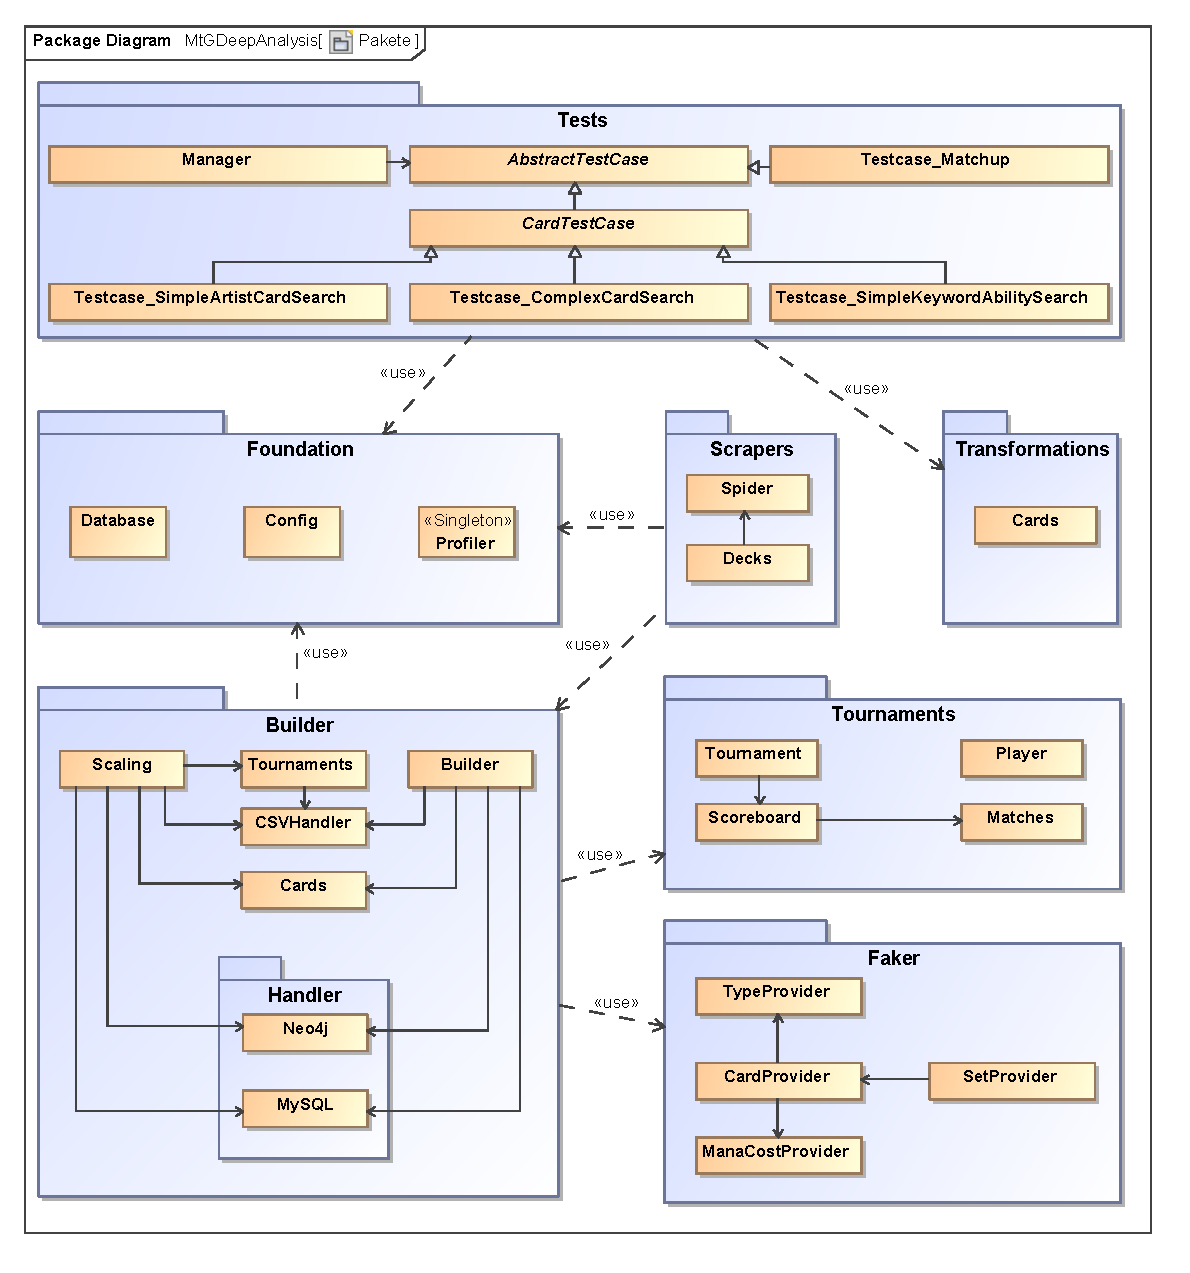
\includegraphics[width=\textwidth]{gfx/sw-components.eps}
    \caption{Software-Komponenten}
    \label{fig:sw-components}
\end{figure}

\begin{description}
    \item[Tests]  \hfill \\
    Enthält die konkreten Testfälle und einen Manager um diese auszuführen
    
    \item[Foundation]  \hfill \\
    Enthält das Grundgerüst, welches von den meisten anderen Paketen benutzt wird
     
    \item[Scrapers]  \hfill \\
    Ist dafür zuständig Decks von mtgtop8 \footnote{\url{http://mtgtop8.com/}} herunterzuladen, um einen Datensatz für Decks zu erstellen
    
    \item[Transformations]  \hfill \\
    Ist zuständig für das Transformieren von Daten in eine vorgegebene Datenstruktur
    
    \item[Builder] \hfill \\
    Ist zuständig für das erstellen und befüllen der Datenbanken
    
    \item[Builder.Handlers]  \hfill \\
    Enthält die Implementierungen für die konkreten Datenbanken
    
    \item[Tournaments]  \hfill \\
    Enthält Datenstrukturen und Algorithmen um Turniere nach dem Schweizer-System zu erstellen und auszuführen
    
    \item[Faker]  \hfill \\
    Ist zuständig für die Erstellung von Dummy-Daten, um die Skalierung der Datenbanken zu testen
\end{description}

\subsection{Beschreibung der Schnittstellen}
%%%%%%%%%%%%%%%%%%%%%%%%%%%%%%%%%%%%%%%%%%%
% Beschreibung der Packet Schnittstellen. %
%%%%%%%%%%%%%%%%%%%%%%%%%%%%%%%%%%%%%%%%%%%
\subsubsection*{Tests}
Die Komponente \verb|Tests| nutzt die folgenden Schnittstellen:
\begin{description}
    \item[Foundation] wird genutzt, um ein Datenbank-Verbindungen zu erstellen und mit dem \verb|Profiler| die Laufzeit und Speicherverbrauch zu messen
    \item[Transformations] wird genutzt, um die ausgelesenen Daten in eine passende Datenstruktur zu überführen
\end{description}

\subsubsection*{Scrapers}
Die Komponente \verb|Scrapers| nutzt die folgenden Schnittstellen:
\begin{description}
    \item[Foundation] wird genutzt, um auf die Konfiguration zuzugreifen
    \item[Builder] wird genutzt, um die Decks in \ac{CSV} Dateien zu speichern
\end{description}

\subsubsection*{Builder}
Die Komponente \verb|Builder| nutzt die folgenden Schnittstellen:
\begin{description}
    \item[Foundation] wird genutzt, um ein Datenbank-Verbindungen zu erstellen
    \item[Tournaments] wird genutzt, um Turnierdaten basierend auf den heruntergeladenen Decks zu erstellen
    \item[Faker] wird genutzt, um ein Dummy-Daten für die Skalierungstests zu erstellen und zu importieren
\end{description}

